% Created 2021-06-01 Tue 17:41
% Intended LaTeX compiler: pdflatex
\documentclass[presentation,aspectratio=169]{beamer}
\usepackage[utf8]{inputenc}
\usepackage[T1]{fontenc}
\usepackage{graphicx}
\usepackage{grffile}
\usepackage{longtable}
\usepackage{wrapfig}
\usepackage{rotating}
\usepackage[normalem]{ulem}
\usepackage{amsmath}
\usepackage{textcomp}
\usepackage{amssymb}
\usepackage{capt-of}
\usepackage{hyperref}
\usepackage{bm}
\usepackage{tikz}
\usetheme{Madrid}
\author{Heng Xiao}
\date{\today}
\title{Invariance of Vector-Cloud Neural Network}
\title[Invariance in VCNN]{Invariance of Vector-Cloud Neural Network}
\author[H. Xiao]{Heng Xiao}
\institute[Virginia Tech]{Virginia Tech \vspace{1em} \\ \emph{Joint work with}: \\  Xuhui Zhou (Virginia Tech) \\ Jiequn Han (Princeton) \\ Ruiying Xu (Delft)}
\hypersetup{
 pdfauthor={Heng Xiao},
 pdftitle={Invariance of Vector-Cloud Neural Network},
 pdfkeywords={},
 pdfsubject={},
 pdfcreator={Emacs 27.2 (Org mode 9.4.4)}, 
 pdflang={English}}
\begin{document}

\maketitle


\section{Invariance of VCNN}
\label{sec:orgba2f479}

\begin{frame}[label={sec:orge226025}]{Problem Statement}
\begin{block}{Overview}
\begin{itemize}
\item We aim to find a mapping from the cloud (\(\tikz \draw (0,0) ellipse
  (6pt and 3pt);\)) to a cloud center (\(\color{blue} \star\)).

\item The cloud has \(n\) points (\(\bullet\)), each with a point \(\mathbf{q}\)
attached to it.

\item The cloud is thus
\(\mathcal{Q} = {[ \mathbf{q}_1^\top, \mathbf{q}_2^\top, \ldots, \mathbf{q}_n^\top]}\).
\end{itemize}

\begin{center}
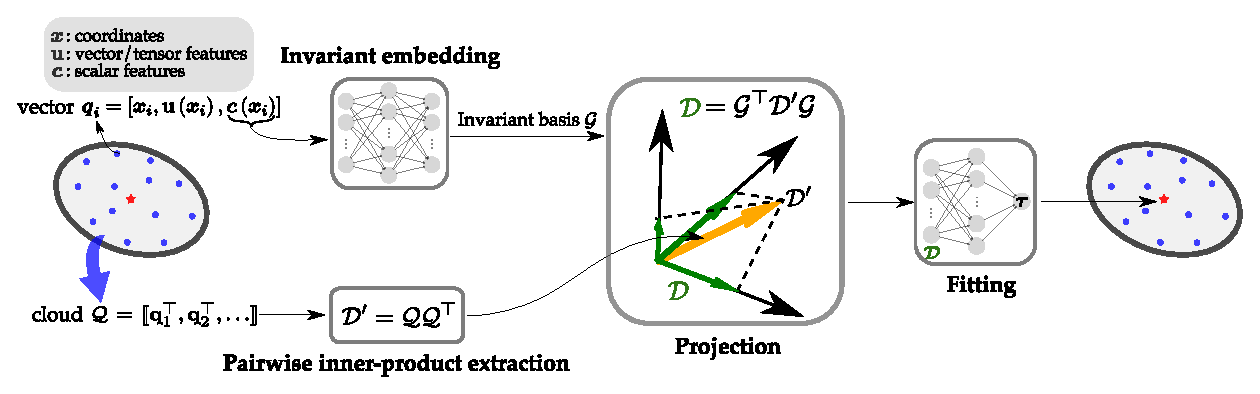
\includegraphics[width=.9\linewidth]{./figs/vcnn.pdf}
\end{center}
\end{block}
\end{frame}

\begin{frame}[label={sec:orgf4e70e5}]{Nomenclature}
\begin{block}{Nomenclature (with example values)}
\begin{itemize}
\item Number of points in cloud: \(n =100\); index \(i\) and
\(i' = 1, \cdots, n\)

\item Number of features \(\ell = 11\); index \(j = 1, \cdots, \ell\)

\item Number of encoding functions \(m=64\), index \(k = 1, \cdots, m\)
\end{itemize}
\end{block}
\end{frame}

\begin{frame}[label={sec:org7daee78}]{Nomenclature - cont.}
\begin{block}{Example dimension of variable}
\begin{itemize}
\item Feature vector for each point:
\(\mathbf{q} \in \mathbb{R}^{11 \times 1}\)

\item Cloud feature matrix: \(\mathcal{Q} \in \mathbb{R}^{100 \times 11}\)

\item Embedding function (64 encoded values for each point)
\(\mathcal{G} \in \mathbb{R}^{100 \times 64}\)

\item Embedded feature matrix: \(\mathcal{G} \in \mathbb{R}^{64 \times 64}\)

\item Reduced embedded matrix
\(\mathcal{G}^\star \in \mathbb{R}^{64 \times 4}\) (keeping only the
first \(m'=4\) columns for compactness).
\end{itemize}
\end{block}
\end{frame}

\begin{frame}[label={sec:org5d61bcd}]{Translational and Galilean Invariance}
Translational and Galilean invariance is straightforward:

\begin{itemize}
\item Use only the \emph{relative} coordinates of the points, not the absolute  locations.

\item Use only the \emph{relative} velocities (for Galilean invariance).
\end{itemize}
\end{frame}


\begin{frame}[label={sec:org0d58ec1}]{Rotational Invariance: First Attempt}
Pairwise projection among the points can remove dependence on coordinate orientation.

\begin{block}{Rotational Invariance with Pairwise Inner Product}
\begin{itemize}
\item Use only the \(\mathbf{q}_i^\top \mathbf{q}_{i'}\), where
\(i, i' = 1 \ldots n\).

\item Hence, \(\mathcal{D}' = \mathcal{Q}^\top  \mathcal{Q}\) is a rotational
invariant feature matrix.

\item \(\mathcal{D}'\) Lacks Permutational Invariance

\item Write
\(\mathcal{D}'_{i i'} = \sum_{j=1}^{\ell} \mathcal{Q}_{ij} \mathcal{Q}_{ji'}\)
(\(i\) and \(i'\) are cloud point indices, and \(j\) is feature index).

\item \(\mathcal{D}'\) would switch rows and columns if the \(n\) points are
permutated (i.e., the numbering is switched).
\end{itemize}
\end{block}

How to achieve permutational invariance?
\end{frame}

\begin{frame}[label={sec:orgbcb1911}]{Permutational Invariance - General}
\begin{exampleblock}{Examples}
 Heuristics: A function where all arguments have the same status
is permutational variant, e.g.,

\begin{itemize}
\item \(f(x_1, x_2, x_3) = \frac{1}{3}(x_1 + x_2 + x_3)\)

\item \(f(x_1, x_2, x_3) = \frac{1}{3}(x_1 + x_2 + x_3) + x_1 x_2 x_3 + x_1 x_2 + x_2 x_3 + x_1 x_3\)
\end{itemize}
\end{exampleblock}

\begin{alertblock}{Counter-Examples:}
These functions are \alert{not} permutational variant:

\begin{itemize}
\item \(f(x_1, x_2, x_3) = x_1(x_2+x_3)\)

\item \(f(x_1, x_2, x_3) = (x_1+x_2 - x_3)\)
\end{itemize}

The arguments have different status in the function.
\end{alertblock}
\end{frame}

\begin{frame}[label={sec:org303b9b4}]{Permutational Invariance}
Summation over all points can achieve permutational invariance Define a
function that depends only on the set of vectors
\(\{\mathbf{q}_i\}_{i=1}^n\) and .

\begin{itemize}
\item Introduce a set of \(m\) functions \(\{\phi_k(\mathbf{c}_i)\}_{k=1}^m\),
where scalars \(\mathbf{c}_i\) is part of feature vector
\(\mathbf{q}_i\), and \(k=1, \ldots, m\) is the embedding function index:
\[
   \mathcal{L}_{k j} = \frac1n \sum^{n}_{\color{red} i=1} \phi_k(\mathbf{c}_{\color{red} i}) \mathcal{Q}_{{\color{red} i}j}
   \]
\end{itemize}

Note

\begin{itemize}
\item Inner product (contraction) between \(\bm{\phi}\) and \(\mathcal{Q}\)
removed dependence on point ordering (index \(i\), red above).

\item This is evident as index \(i\) disappeared in the results
\(\mathcal{L}_{k j}\) after the contraction.
\end{itemize}
\end{frame}

\begin{frame}[label={sec:orgc335502}]{Rotational Invariance: Final Attempt}
\begin{block}{\(\mathcal{L}\) is Permutational Invariant}
\begin{itemize}
\item Order-removing transformation:
\(\mathcal{L}_{k j} = \frac{1}{n} \sum_{i=1}^n \phi_k(\mathbf{c}_i) \,  \mathcal{Q}_{ij}\)

\item Or in matrix form: \(\mathcal{L}=\frac{1}{n} G^\top \mathcal{Q}\) with
\(\mathcal{G}_{k i} = \phi_k(\mathbf{c}_i)\).
\end{itemize}
\end{block}

\begin{block}{Achieve Rotational Invariance}
\begin{itemize}
\item \(\mathcal{L}\) is obtained by rotating and scaling \(\mathcal{Q}\)

\item \(\mathcal{D} = \mathcal{L} \mathcal{L}^{\top} \equiv \frac{1}{n^2}\mathcal{G}^\top \mathcal{Q} \mathcal{Q}^\top \mathcal{G}\)
is rotational invariant

\item Note that \(\mathcal{D}\) is also translational and permutational
invariant because \(\mathcal{L}\) is.
\end{itemize}
\end{block}
\end{frame}

\begin{frame}[label={sec:org20ab6c4}]{Compact Representation}
We have transformed cloud feature \(\mathcal{Q}\)
to invariant \(\mathcal{D}\):
\[
\mathcal{D} = \mathcal{L} \mathcal{L}^{\top} \equiv
\frac{1}{n^2}\mathcal{G}^\top \mathcal{Q} \mathcal{Q}^\top\ \mathcal{G}
\]

\begin{block}{Example Problem Size}
\begin{itemize}
\item Cloud has \(n=100\) points.

\item Each point has a feature vector of length \(\ell = 11\).

\item We chose \(m = 64\) encoding functions, i.e., size of
\(\bm{\phi} = \{\phi_j\}_{j=1}^{64}\).

\item \(\mathcal{Q}\in \mathbb{R}^{100 \times 11}\) (1100 raw features)

\item \(\Longrightarrow\) \(\mathcal{D}\in \mathbb{R}^{64 \times 64}\) (4096
embedded features)
\end{itemize}
\end{block}

\alert{May not need so many features!}
\end{frame}

\begin{frame}[label={sec:org3a5a3ea}]{Compact Representation}
\begin{block}{Feature Compression}
\begin{itemize}
\item It is desirable to only keep first \(m' \ll m\) columns of
\(\mathcal{D}\) for a more compact encoding.
\item To this end, we define:

\[ \mathcal{D} = \mathcal{L} \mathcal{L}^{\star \top}
  \equiv \frac{1}{n^2}\mathcal{G}^\top \mathcal{Q} \mathcal{Q}^\top
  \mathcal{G}^\star \in \mathbb{R}^{64 \times 4} \]
\end{itemize}
\end{block}

\begin{itemize}
\item \(\mathcal{G}^\star\) is the first \(m'\) columns of \(\mathcal{G}\). We
used \(m' = 4\) in our paper.
\item Thus we have \(m\times m' = 64 \times 4 = 256\) invariant features.
\end{itemize}
\end{frame}

\begin{frame}[label={sec:orgb440440}]{Overview Again}
\begin{center}
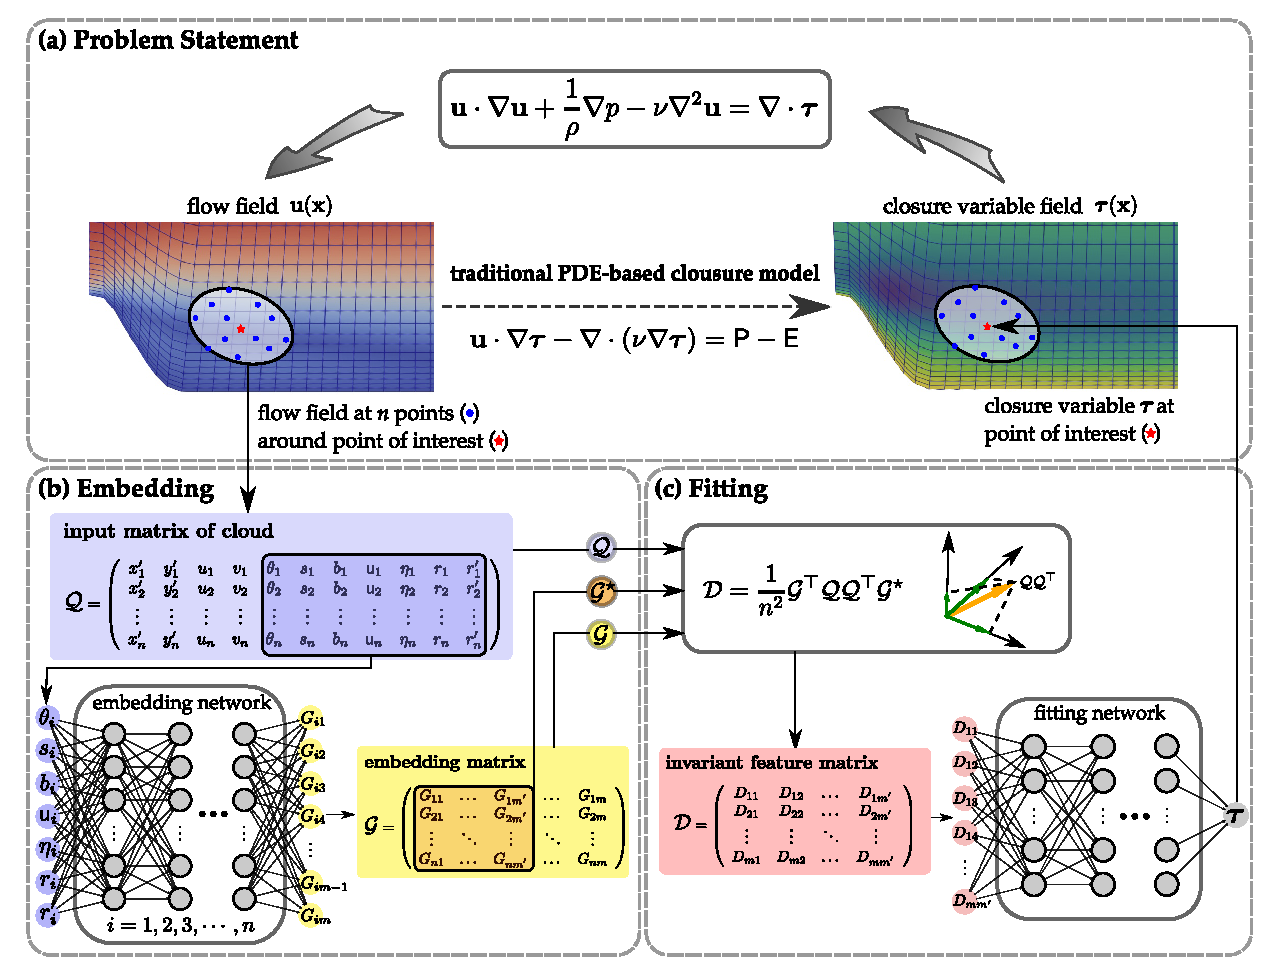
\includegraphics[width=0.75\textwidth]{figs/NN-architecture.eps}
\end{center}
\end{frame}

\section{Invariance with a Minimum Example}
\label{sec:org1867efb}
\end{document}